\section{Energieeichung}

Um eine Aussage über die Energie der von den Präparaten emittierten Strahlung zu machen, muss man erstmal einen Zusammenhang zwischen 
den Kanalnummern des Vierkanalanalysators und den Energiewerte hergestellt werden. Wir nehmen dazu an, dass der Zusammenhang linear sei. Nun bringen wir 
die charakteristischen Linien dreier Präparate mit Kanalnummern in Verbindung. Danach bestimmen 
wir via linearer Regression die Parameter $E_0$  für den y-Achsenabschnitt und $m$ für die Steigung.\\

Die drei verwendeten Präparate/Emissionslinien  sind:
 \begin{table}[h]
    \centering
     \begin{tabular}{lcr}
        Isotop & Energie (MeV) & Kanalnummer \\
        \toprule
         Cs-137 & 0,6616  & 447\\
         Am-241 & 0.0594 & 41\\
         Co-60 & 1.1732 & 792\\
     \end{tabular}
     \caption{Zur Energieeichung verwendete Spektrallinien}
     \label{Eichung}
 \end{table}

 Mit linearer Regression erhält man $E_0 = -1386.75067405 \mathrm{ eV}$ und $m = 1483.09394689 \frac{\mathrm{eV}}{\mathrm{Kanal}}$.
 Dabei sieht man sehr gut an Grafik \ref{Eichgerade}, dass die Annahme eines linearen Zusammenhangs gerechtfertigt ist und der Vierkanalanalysators in 
 diesem Bereich linear arbeitet.

 \begin{figure}[ht]
     \centering
     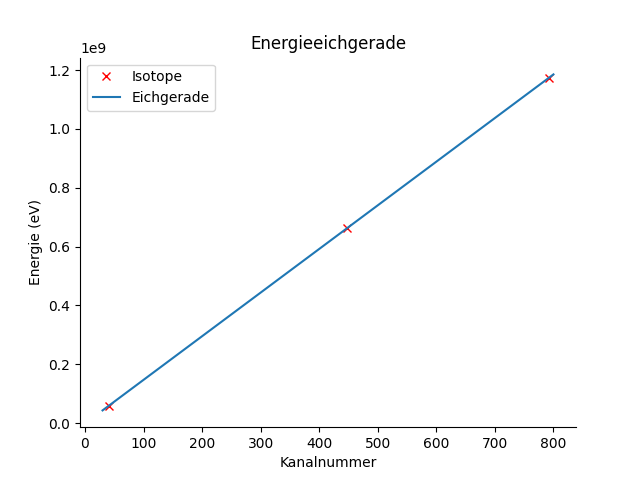
\includegraphics[width = \linewidth]{Bilder/Auswertung/EnergieeichgeradeGamma.png}
     \caption{Eichgerade anhand der oben verwendeten Isotope}
     \label{Eichgerade}
 \end{figure}